\documentclass{article}
\usepackage[utf8]{inputenc}
\usepackage[ngerman]{babel}

% Convenience improvements
\usepackage{csquotes}
\usepackage{enumitem}
\setlist[enumerate,1]{label={\alph*)}}
\usepackage{amsmath}
\usepackage{amssymb}
\usepackage{mathtools}
\usepackage{tabularx}

% Proper tables and centering for overfull ones
\usepackage{booktabs}
\usepackage{adjustbox}

% Change page/text dimensions, the package defaults work fine
\usepackage{geometry}
\usepackage{parskip}

% Drawings
\usepackage{tikz}
\usepackage{forest}

% Adjust header and footer
\usepackage{fancyhdr}
\pagestyle{fancy}
\fancyhead[L]{Algorithms and Data Structures 2 --- \textbf{Assignment 4}}
\fancyhead[R]{Laurenz Weixlbaumer (11804751)}
\fancyfoot[C]{}
\fancyfoot[R]{\thepage}
% Stop fancyhdr complaints
\setlength{\headheight}{12.5pt}

\newcommand{\Deltaop}{\, \Delta\, }
\newcommand{\xor}{\, \oplus\, }

\begin{document}

\begin{enumerate}[label=(\arabic*)]
    \item \phantom{}
    \begin{center}
        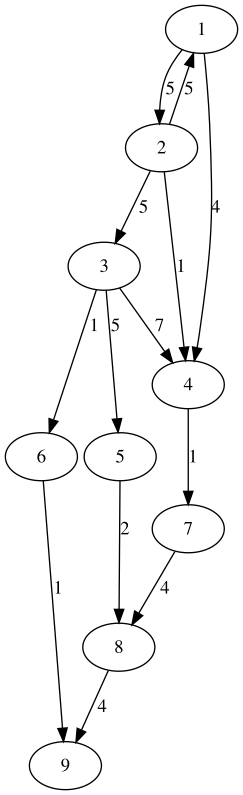
\includegraphics[width=.25\textwidth]{graph1.png}
        \begin{enumerate}
            \item Yes
            \item Yes
            \item 4
            \item 3
            \item 7
            \item cyclic
            \item 0
            \item weakly
            \item no
        \end{enumerate}
    \end{center}

    \item \phantom{}
    \begin{center}
        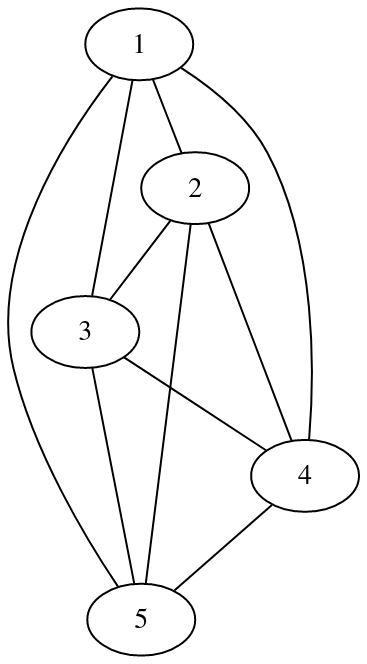
\includegraphics[width=.25\textwidth]{graph2.png}
    \end{center}

    \item \phantom{}
    \begin{center}
        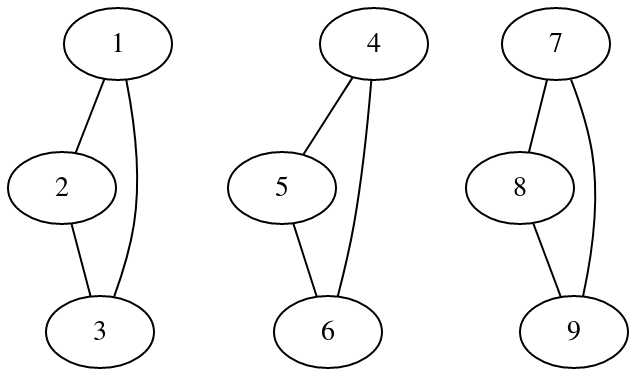
\includegraphics[width=.5\textwidth]{graph3.png}
    \end{center}

    \item \phantom{}
    \begin{center}
        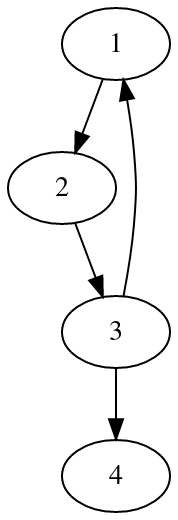
\includegraphics[width=.15\textwidth]{graph4.png}
    \end{center}

    % d6 = 7, d7 = 5, d8 = 1*
    \item \phantom{}
    \begin{center}        
        \begin{tabular}{l l l l}
            1 & [7, 2, 6] & 2 & [1] \\
            2 & [5, 1*, 4] & 1* & [1, 2] \\
            1* & [] & 2 (up) & [1, 2, 1*] \\
            2 & [5, 1*, 4] & 4 & [1, 2, 1*] \\
            4 & [] & 2 (up) & [1, 2, 1*, 4] \\
            2 & [5, 1*, 4] & 5 & [1, 2, 1*, 4] \\
            5 & [0] & 0 & [1, 2, 1*, 4, 5] \\
            0 & [] & 5 (up) & [1, 2, 1*, 4, 5, 0] \\
            5 & [0] & 2 (up) & [1, 2, 1*, 4, 5, 0] \\
            2 & [5, 1*, 4] & 1 (up) & [1, 2, 1*, 4, 5, 0] \\
            1 & [7, 2, 6] & 6 & [1, 2, 1*, 4, 5, 0] \\
            6 & [] & 1 (up) & [1, 2, 1*, 4, 5, 0, 6] \\
            1 & [7, 2, 6] & 7 & [1, 2, 1*, 4, 5, 0, 6] \\
            7 & [5] & 1 (up) & [1, 2, 1*, 4, 5, 0, 6, 7] \\
        \end{tabular}
    \end{center}
\end{enumerate}

\end{document}
